\documentclass[a4paper,oneside,12pt]{extarticle}

\usepackage[utf8]{inputenc}
\usepackage[english]{babel}
\usepackage{amssymb,amsthm,mathtools,enumitem,geometry,hyperref,booktabs}
\usepackage{graphicx}
\usepackage{xcolor}
\usepackage{tikz}
\usetikzlibrary{calc,patterns,decorations.pathreplacing}
\usepackage{tikz-cd}
\usepackage{pgfplots}
\usepgfplotslibrary{fillbetween}
\pgfplotsset{compat=1.18}
\usepackage{float}

\geometry{lmargin=15mm,rmargin=15mm,tmargin=10mm,bmargin=10mm,includeheadfoot}
\pagestyle{plain}
\frenchspacing

\theoremstyle{plain}
\newtheorem{proposition}{Proposition}
\newtheorem{lemma}[proposition]{Lemma}

\theoremstyle{definition}
\newtheorem{definition}[proposition]{Definition}
\newtheorem{example}[proposition]{Example}

\theoremstyle{remark}
\newtheorem{remark}[proposition]{Remark}

\newcommand*{\E}{\mathbb{E}}
\newcommand*{\Var}{\mathrm{Var}}
\newcommand*{\mP}{\mathbb{P}}
\newcommand*{\mR}{\mathbb{R}}
\newcommand*{\mbF}{\mathcal{F}}
\newcommand*{\ve}{\varepsilon}




\begin{document}
\begin{titlepage}
\begin{center}

{\footnotesize\scshape\color{gray}
Working Notes in Quantitative Risk and Modeling
}

\vfill

{\LARGE\bfseries Homoscedasticity and Its Testing:\\[4pt]
From Conditional Expectation to the Breusch--Pagan Test}

\vspace{36pt}

{\normalsize Boris Garbuzov}

\vfill

{\Large\bfseries Part~3~/~12}

\vspace{6pt}

{\Large\bfseries Maximum Likelihood Estimation: A Worked Example}

\vfill

{\small July 2026}

\end{center}
\end{titlepage}

\setcounter{tocdepth}{2}
\tableofcontents
\newpage
\section{Maximum Likelihood Estimation: Worked Examples}
\label{sec:mle_worked_examples}
%====================================================================

This chapter works through MLE explicitly in two contrasting
families: the regular $\mathcal{N}(\mu,1)$ family, where the MLE
is found by setting the score to zero, and the non-regular
$\mathrm{U}[0,\theta]$ family, where the MLE is the sample maximum.

\subsection{Worked example: $\mathcal{N}(\mu,1)$ from end to end}
\label{sec:normal_example_end_to_end}
%--------------------------------------------------------------------

We close the Score and Fisher Information chapter (Part~2) by working a single
family --- the unit-variance location-normal $\mathcal{N}(\mu,1)$
--- through every construction of the last three chapters: density,
pre-likelihood, log-likelihood, the randomisation of the index, the
pre-score, the score, and the integral identity $\E[s]=0$.  The
example is small enough to compute explicitly, so the abstract
pattern becomes concrete.  These notes follow the Probabilist's
worksheet of May~15, 2026.

\paragraph{Step 1.\ The density family.}
Take $\theta = \mu \in \mathbb{R}$, scalar.  The density is
\[
  f_\mu(x) \;=\; \frac{1}{\sqrt{2\pi}}\,\exp\!\Bigl(-\tfrac{(x-\mu)^2}{2}\Bigr)
  \;=\; \varphi(x-\mu),
\]
where $\varphi$ denotes the standard normal density.  For a fixed
value $\mu_0$, $f_{\mu_0}$ is a bell curve in $x$ centred at $\mu_0$,
of unit area.

\begin{center}
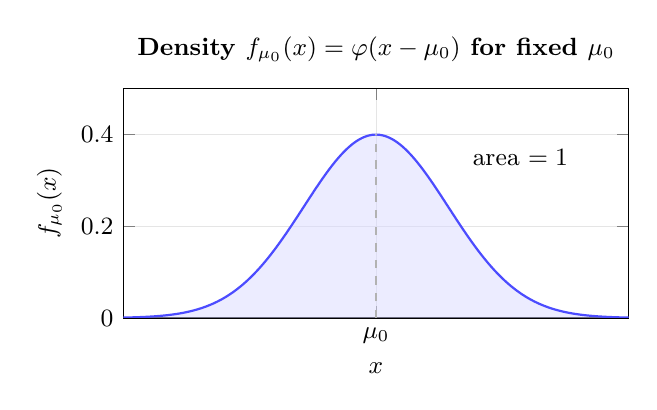
\begin{tikzpicture}
\begin{axis}[
  width=8cm, height=4.5cm,
  xlabel={$x$}, ylabel={$f_{\mu_0}(x)$},
  title={Density $f_{\mu_0}(x)=\varphi(x-\mu_0)$ for fixed $\mu_0$},
  xmin=-3.5, xmax=3.5, ymin=0, ymax=0.50,
  domain=-3.5:3.5, samples=200,
  grid=both, grid style={line width=0.3pt,draw=gray!20},
  tick label style={font=\small},
  title style={font=\small\bfseries},
  label style={font=\small},
  xtick={0}, xticklabels={$\mu_0$},
]
\addplot[thick,blue!70,name path=f]{exp(-x^2/2)/sqrt(2*3.14159)};
\addplot[name path=zero,draw=none]{0};
\addplot[blue!15,opacity=0.5] fill between[of=f and zero];
\addplot[dashed,gray!60] coordinates {(0,0)(0,0.40)};
\node[font=\small] at (axis cs:2.0,0.35) {area $=1$};
\end{axis}
\end{tikzpicture}
\end{center}

\paragraph{Step 2.\ The pre-likelihood.}
For a fixed observation $x_1$,
\[
  L_{x_1}(\mu) \;=\; \varphi(x_1-\mu)
\]
is the pre-likelihood as a function of $\mu$.  It is also a bell
curve, now along the $\mu$-axis and centred at $\mu_0 = x_1$.  This
is the location-normal coincidence (the location-normal symmetry remark (Part~2)):
the density slice and the pre-likelihood slice look the same.

\begin{center}
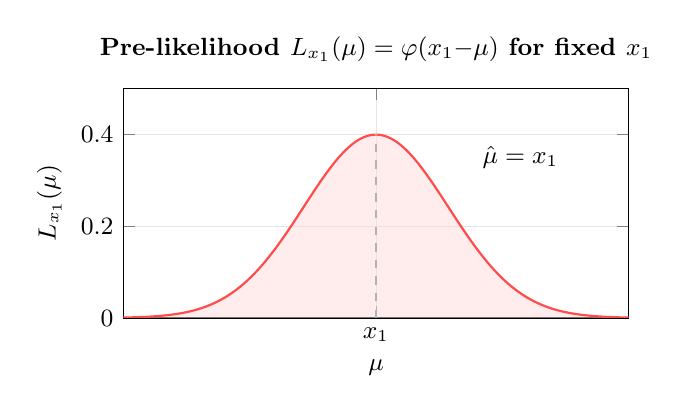
\begin{tikzpicture}
\begin{axis}[
  width=8cm, height=4.5cm,
  xlabel={$\mu$}, ylabel={$L_{x_1}(\mu)$},
  title={Pre-likelihood $L_{x_1}(\mu)=\varphi(x_1{-}\mu)$ for fixed $x_1$},
  xmin=-3.5, xmax=3.5, ymin=0, ymax=0.50,
  domain=-3.5:3.5, samples=200,
  grid=both, grid style={line width=0.3pt,draw=gray!20},
  tick label style={font=\small},
  title style={font=\small\bfseries},
  label style={font=\small},
  xtick={0}, xticklabels={$x_1$},
]
\addplot[thick,red!70,name path=g]{exp(-x^2/2)/sqrt(2*3.14159)};
\addplot[name path=zero2,draw=none]{0};
\addplot[red!15,opacity=0.5] fill between[of=g and zero2];
\addplot[dashed,gray!60] coordinates {(0,0)(0,0.40)};
\node[font=\small] at (axis cs:2.0,0.35) {$\hat\mu=x_1$};
\end{axis}
\end{tikzpicture}
\end{center}

\paragraph{Step 3.\ The bivariate surface.}
The two slices live on one surface
\[
  h(x,\mu) \;=\; \varphi(x-\mu),
\]
which depends on its two arguments only through the difference
$x-\mu$.  The ridge of the surface is the line $x = \mu$.

\begin{center}
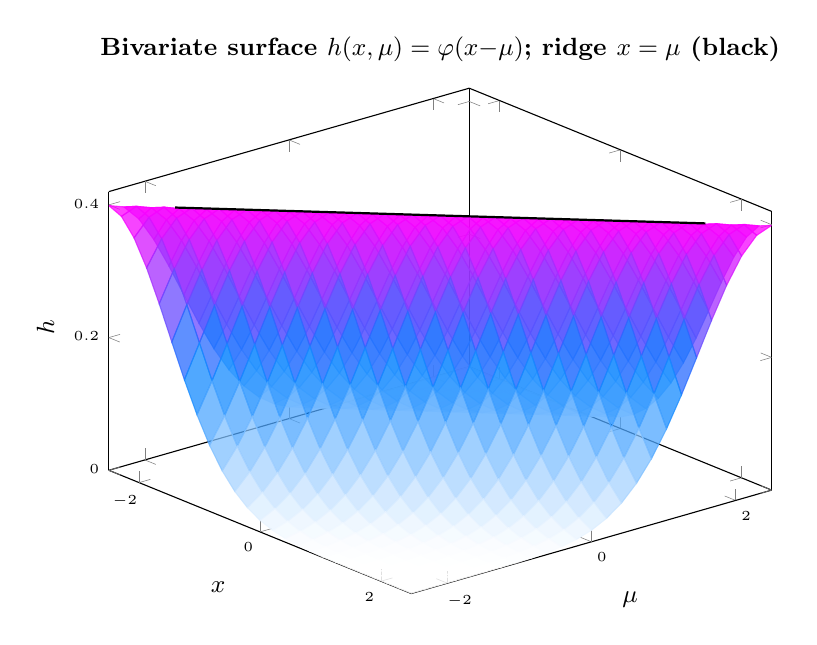
\begin{tikzpicture}
\begin{axis}[
  width=10cm, height=8cm,
  xlabel={$x$}, ylabel={$\mu$}, zlabel={$h$},
  title={Bivariate surface $h(x,\mu)=\varphi(x{-}\mu)$; ridge $x=\mu$ (black)},
  xmin=-2.5, xmax=2.5, ymin=-2.5, ymax=2.5, zmin=0, zmax=0.42,
  domain=-2.5:2.5, y domain=-2.5:2.5, samples=25,
  view={50}{30},
  colormap/cool,
  title style={font=\small\bfseries},
  label style={font=\small},
  tick label style={font=\tiny},
]
\addplot3[surf,opacity=0.75,shader=flat corner]
  {exp(-(x-y)^2/2)/sqrt(2*3.14159)};
\addplot3[thick,black,domain=-2:2,samples=50]
  (x,x,{exp(0)/sqrt(2*3.14159)});
\end{axis}
\end{tikzpicture}
\end{center}

\paragraph{Step 4.\ The pre-log-likelihood.}
Take the log on the positivity set (all of $\mathbb{R}$ here,
since $f_\mu > 0$ everywhere):
\[
  \ell_x(\mu) \;=\; \log h(x,\mu)
  \;=\; -\tfrac{1}{2}\log(2\pi) - \tfrac{1}{2}(x-\mu)^2.
\]
A downward parabola in $\mu$ with vertex at $\mu = x$ and peak
value $-\tfrac{1}{2}\log(2\pi)$ (the same value at every observation
$x$ --- a peculiarity of the location-normal family).

\begin{center}
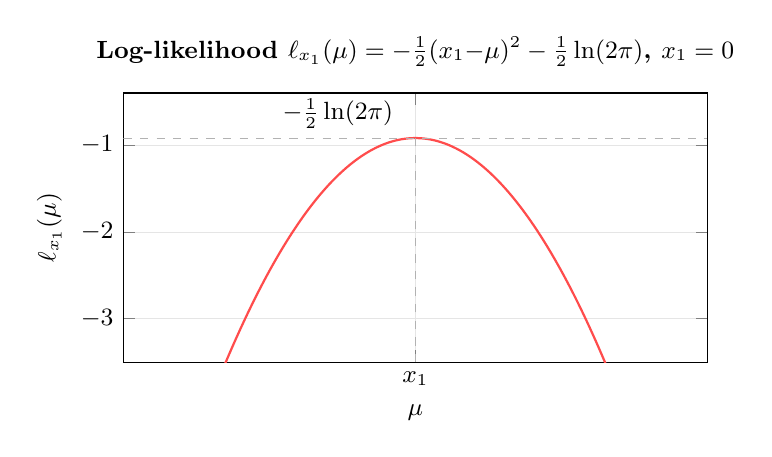
\begin{tikzpicture}
\begin{axis}[
  width=9cm, height=5cm,
  xlabel={$\mu$}, ylabel={$\ell_{x_1}(\mu)$},
  title={Log-likelihood $\ell_{x_1}(\mu)=-\tfrac{1}{2}(x_1{-}\mu)^2-\tfrac{1}{2}\ln(2\pi)$,\ $x_1=0$},
  xmin=-3.5, xmax=3.5, ymin=-3.5, ymax=-0.4,
  domain=-3.5:3.5, samples=200,
  grid=both, grid style={line width=0.3pt,draw=gray!20},
  tick label style={font=\small},
  title style={font=\small\bfseries},
  label style={font=\small},
  xtick={0}, xticklabels={$x_1$},
]
\addplot[thick,red!70]{-x^2/2 - 0.919};
\addplot[dashed,gray!60] coordinates {(0,-3.5)(0,-0.919)};
\addplot[dashed,gray!60] coordinates {(-3.5,-0.919)(3.5,-0.919)};
\node[font=\small,anchor=south east] at (axis cs:-0.15,-0.919)
  {$-\tfrac{1}{2}\ln(2\pi)$};
\node[font=\small,anchor=south] at (axis cs:0,-0.4)
  {vertex: $\hat\mu=x_1$};
\end{axis}
\end{tikzpicture}
\end{center}

\paragraph{Step 5.\ Connecting $\Omega$: random parabolas.}
Now treat the observation as a random variable $X(\omega) \sim
\mathcal{N}(\mu_0, 1)$ for some true parameter $\mu_0 \in \mathbb{R}$.
Each $\omega$ produces one realised observation $x = X(\omega)$ and
hence one realised pre-log-likelihood --- a single downward parabola
with vertex at that observed $x$.  Sampling many $\omega$'s
materialises a \emph{cloud of random parabolas}, each centred at
its own $X(\omega)$.

The parabolas are denser where the observations are denser.  Since
$X \sim \mathcal{N}(\mu_0, 1)$, the observations cluster around
$\mu_0$ and thin out in the tails, so the vertices of the random
parabolas cluster around $\mu_0$ and thin out in the tails as well.
This is the picture on page~2 of the worksheet: an $\Omega$-cloud
on top, arrows pointing down to a handful of realised $x_i$'s along
the $\mu$-axis, and a fan of downward parabolas with vertices at
those $x_i$'s.  The randomness of the log-likelihood is exactly this
cloud of parabolas indexed by $\omega$.

\begin{remark}[The MLE for a single observation]
For one observation $x$, $\ell_x(\mu) = -\tfrac{1}{2}(x-\mu)^2 + C$
is maximised at $\hat\mu = x$.  So
\[
  \widehat{\mu}_{\text{MLE}}(X(\omega)) \;=\; X(\omega).
\]
The MLE is the observation itself.  This is the simplest possible
estimator and a sanity check: in this family, the data \emph{is}
the maximum-likelihood guess for the location.
\end{remark}

\begin{center}
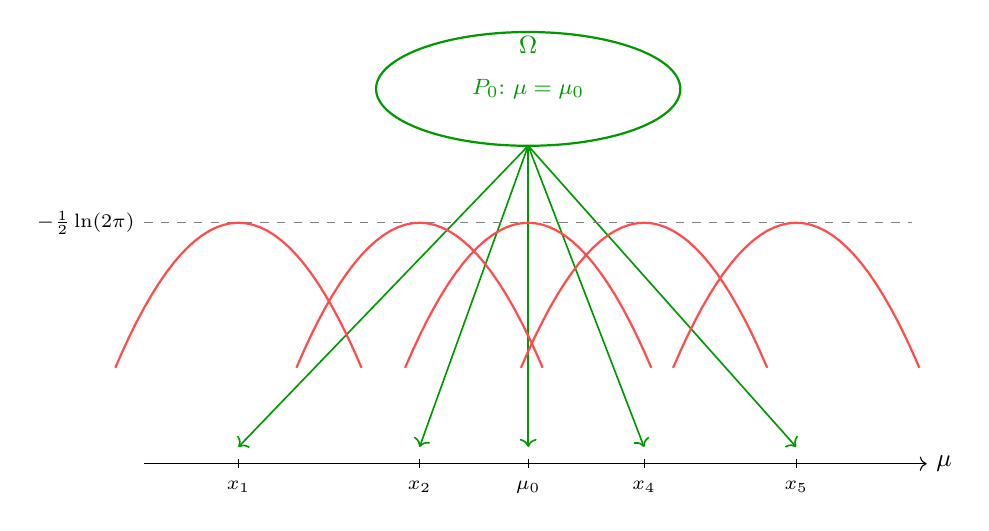
\begin{tikzpicture}[font=\small,yscale=0.85,xscale=0.92]
% Omega cloud
\draw[thick,green!60!black] (0,5.6) ellipse (2.1cm and 0.85cm);
\node[green!60!black] at (0,6.25) {$\Omega$};
\node[green!60!black,font=\footnotesize] at (0,5.6)
  {$P_0{:}\ \mu=\mu_0$};
% Arrows from Omega to realisations
\foreach \xi in {-4,-1.5,0,1.6,3.7}{
  \draw[->,green!60!black,semithick] (0,4.75) -- (\xi,0.25);
}
% mu-axis
\draw[->] (-5.3,0) -- (5.5,0) node[right]{$\mu$};
\node[below,font=\scriptsize] at (-4,-0.12)  {$x_1$};
\node[below,font=\scriptsize] at (-1.5,-0.12){$x_2$};
\node[below,font=\scriptsize] at (0,-0.12)   {$\mu_0$};
\node[below,font=\scriptsize] at (1.6,-0.12) {$x_4$};
\node[below,font=\scriptsize] at (3.7,-0.12) {$x_5$};
\foreach \xi in {-4,-1.5,0,1.6,3.7}{
  \draw (\xi,-0.07)--(\xi,0.07);
}
% peak level
\draw[dashed,gray] (-5.3,3.6)--(5.3,3.6);
\node[left,font=\scriptsize] at (-5.3,3.6){$-\tfrac{1}{2}\ln(2\pi)$};
% downward parabolas
\foreach \cx in {-4,-1.5,0,1.6,3.7}{
  \draw[red!70,thick,domain={\cx-1.7}:{\cx+1.7},samples=35,variable=\t]
    plot(\t,{3.6-0.75*(\t-\cx)*(\t-\cx)});
}
\end{tikzpicture}
\end{center}

\paragraph{Step 6.\ The pre-score.}
Differentiate $\ell_x$ in $\mu$:
\[
  s(x,\mu) \;=\; \frac{\partial}{\partial\mu}\,\ell_x(\mu)
  \;=\; \frac{\partial}{\partial\mu}\!\left[-\tfrac{1}{2}(x-\mu)^2\right]
  \;=\; (x-\mu).
\]
The pre-score is the affine function $(x,\mu) \mapsto x - \mu$.
At any fixed $x_1$, it is a downward-sloping line in $\mu$, passing
through zero at $\mu = x_1$.  At any fixed $\mu_0$, it is an
upward-sloping line in $x$, passing through zero at $x = \mu_0$.

\begin{center}
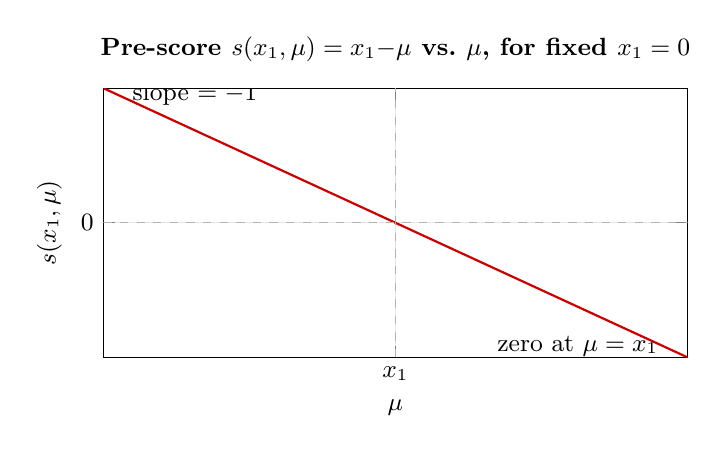
\begin{tikzpicture}
\begin{axis}[
  width=9cm, height=5cm,
  xlabel={$\mu$}, ylabel={$s(x_1,\mu)$},
  title={Pre-score $s(x_1,\mu)=x_1{-}\mu$ vs.\ $\mu$, for fixed $x_1=0$},
  xmin=-3, xmax=3, ymin=-3, ymax=3,
  domain=-3:3, samples=100,
  grid=both, grid style={line width=0.3pt,draw=gray!20},
  tick label style={font=\small},
  title style={font=\small\bfseries},
  label style={font=\small},
  xtick={0}, xticklabels={$x_1$},
  ytick={0},
]
\addplot[thick,red!80!black]{-x};
\addplot[dashed,gray!60] coordinates {(-3,0)(3,0)};
\addplot[dashed,gray!60] coordinates {(0,-3)(0,3)};
\node[font=\small,anchor=south west] at (axis cs:-2.8,2.4)
  {slope $=-1$};
\node[font=\small,anchor=north east] at (axis cs:2.8,-2.3)
  {zero at $\mu=x_1$};
\end{axis}
\end{tikzpicture}
\end{center}

The same affine form $s(x,\mu) = x - \mu$ as a function of two
arguments describes a tilted plane in 3D: a saddle-like ramp that
crosses zero along the ridge $x = \mu$, positive on one side, negative
on the other.  The 3D picture on page~4 of the worksheet shows this
plane intersecting the zero plane along the MLE ridge $x = \mu$.

\begin{center}
\includegraphics[width=0.82\textwidth]{fig_ne_prescoresurface.png}
\end{center}

\paragraph{Step 7.\ The integral identity $\E_{\mu_0}[s] = 0$, geometrically.}
Now fix the true parameter $\mu_0$ and look along the $x$-axis at
fixed $\mu = \mu_0$.  On this slice:
\begin{itemize}
\item the density is $f_{\mu_0}(x) = \varphi(x - \mu_0)$, a bell
  centred at $\mu_0$;
\item the score is $s(x, \mu_0) = x - \mu_0$, a straight line of
  slope $1$ crossing zero at $x = \mu_0$;
\item their product is
  $s(x,\mu_0)\cdot f_{\mu_0}(x) = (x - \mu_0)\,\varphi(x-\mu_0)$,
  an odd function around $\mu_0$.
\end{itemize}
The expected score is the integral of this product:
\[
  \E_{\mu_0}[s(\mu_0)]
  \;=\; \int_{\mathbb{R}} s(x, \mu_0)\,f_{\mu_0}(x)\,dx
  \;=\; \int_{\mathbb{R}} (x-\mu_0)\,\varphi(x-\mu_0)\,dx
  \;=\; 0,
\]
by symmetry: positive and negative areas cancel exactly.

This is the diagram on page~5 of the worksheet: \textbf{green}
density, \textbf{red} score (the straight line crossing zero at
$\mu_0$), \textbf{black} their product (an odd S-curve through
$\mu_0$).  The black curve integrates to zero in Lebesgue measure.


\noindent The bivariate view below shows both surfaces simultaneously: the
green density ridge $h(x,\mu)$ and the red pre-score plane $s(x,\mu)$
share the ridge $x=\mu$, where the score is zero and the density is at its
maximum.  Back-projecting to the fixed slice $\mu=\mu_0$ (the vertical cut)
gives the two curves whose product is the black odd curve in the next plot.

\begin{center}
\includegraphics[width=0.82\textwidth]{fig_ne_combined3d.png}
\end{center}

\medskip
\noindent\textbf{Back to 2D.} Fixing $\mu=\mu_0$ and projecting onto the
$x$-axis yields the three curves below.

\begin{center}
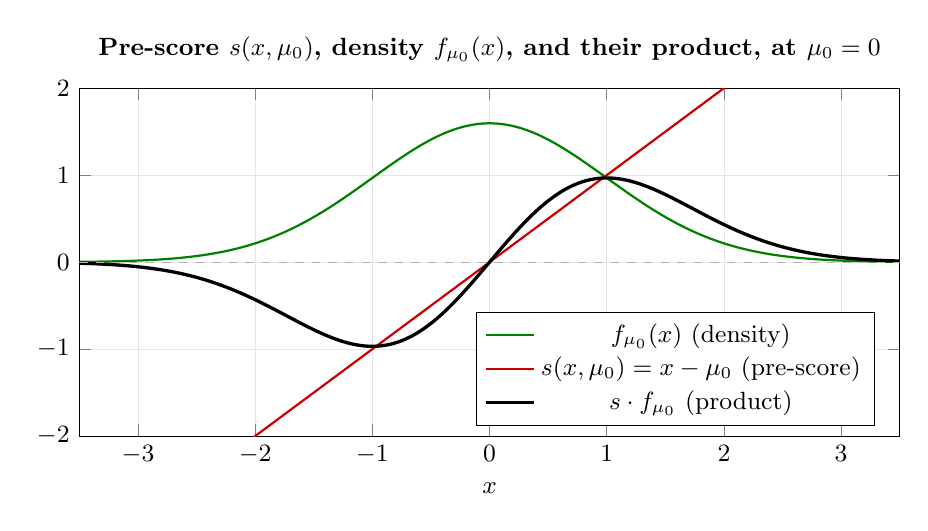
\begin{tikzpicture}
\begin{axis}[
  width=12cm, height=6cm,
  xlabel={$x$},
  title={Pre-score $s(x,\mu_0)$, density $f_{\mu_0}(x)$, and their product, at $\mu_0=0$},
  xmin=-3.5, xmax=3.5, ymin=-2, ymax=2,
  domain=-3.5:3.5, samples=200,
  grid=both, grid style={line width=0.3pt, draw=gray!20},
  tick label style={font=\small},
  title style={font=\small\bfseries},
  label style={font=\small},
  legend pos=south east, legend style={font=\small},
]
% density (green), rescaled for visibility
\addplot[thick, green!50!black] {exp(-x^2/2)/sqrt(2*3.14159)*4};
% score (red): s = x - mu0 = x
\addplot[thick, red!80!black] {x};
% product: (x-mu0)*phi(x-mu0), rescaled for visibility
\addplot[thick, black, very thick]
  {x * exp(-x^2/2)/sqrt(2*3.14159)*4};
% horizontal zero line
\addplot[dashed, gray!60] coordinates {(-3.5,0)(3.5,0)};
\legend{{$f_{\mu_0}(x)$ (density)}, {$s(x,\mu_0)=x-\mu_0$ (pre-score)},
        {$s\cdot f_{\mu_0}$ (product)}}
\end{axis}
\end{tikzpicture}
\end{center}

\noindent\emph{Note on the rescaling:} the density $f_{\mu_0}$ and
the product $s\cdot f_{\mu_0}$ have been multiplied by $4$ in this
plot so that all three curves sit on a comparable vertical scale.
The shape of each curve, and the symmetry that makes the product
integrate to zero, are not affected.

By symmetry of the $\mathcal{N}(\mu_0, 1)$ density around $\mu_0$,
this cancellation holds for \emph{every} $\mu_0 \in \mathbb{R}$,
not just $\mu_0 = 0$.  The score identity $\E_\mu[s(\mu)] = 0$ is
not a deep theorem for this family --- it is an immediate visual
consequence of the symmetry of the bell curve.

\paragraph{Step 8.\ The same identity as integration that cancels the denominator.}
There is a parallel route to the same identity that is worth
flagging, since it generalises beyond the symmetric case.  The
pre-score is
\[
  s(x,\mu) \;=\; \frac{\partial_\mu h(x,\mu)}{h(x,\mu)}.
\]
Taking the expectation against the density $f_\mu = h(\cdot, \mu)$
multiplies the pre-score by $h$ in the integrand, and the
denominator cancels:
\[
  \E_\mu[s(\mu)]
  \;=\; \int s(x, \mu)\,h(x, \mu)\,dx
  \;=\; \int \frac{\partial_\mu h(x,\mu)}{h(x,\mu)}\cdot h(x,\mu)\,dx
  \;=\; \int \partial_\mu h(x,\mu)\,dx
  \;=\; 0.
\]
The final step is Property~3 of
the Density and Likelihood chapter (Part~2).  So the cancellation is
not specific to the symmetry of the normal: it follows from the
fact that $h$ integrates to one in $x$ for every $\mu$.  The normal
case just gives a particularly transparent picture in which both
arguments --- symmetry and Property~3 --- yield the same answer.

\paragraph{What this example gave us.}
A single family, computed step by step, instantiates everything from
the Density/Likelihood and Score chapters (Part~2):
the bivariate surface, two kinds of slices, log transform, random
indexing via $\omega$ producing a cloud of parabolas, the affine
pre-score $x - \mu$, the saddle-shaped score surface, and the
integral $\E[s] = 0$ realised as the area under an odd black curve.
The next subsection extends the same example to $n > 1$ observations,
where the sample mean $\bar x$ enters as a sufficient statistic and
the score acquires its characteristic $\bar x - \mu$ form.

%--------------------------------------------------------------------
\subsection{Worked example continued: $n$ observations}
\label{sec:normal_example_n_obs}
%--------------------------------------------------------------------

We continue the $\mathcal{N}(\mu,1)$ example to the case of a
sample $\mathbf{x} = (x_1,\ldots,x_n)$ of size $n>1$, i.i.d.\ from
$\mathcal{N}(\mu,1)$.  The aim is twofold: to see how the bivariate
surface picture extends to dimension $n+1$; and to verify the
identity $\E_\mu[s] = 0$ by direct calculation, in three rounds of
increasing complexity, following the Probabilist's worksheet of
May~16, 2026.

\paragraph{Step 9.\ The joint density and joint log-likelihood.}
By independence,
\[
  h(x_1,\ldots,x_n; \mu)
  \;=\; \prod_{i=1}^n \varphi(x_i - \mu)
  \;=\; \frac{1}{(2\pi)^{n/2}}\,
  \exp\!\Bigl(-\tfrac{1}{2}\sum_{i=1}^n (x_i - \mu)^2\Bigr).
\]
Taking the log,
\[
  \ell(x_1,\ldots,x_n; \mu)
  \;=\; -\tfrac{n}{2}\log(2\pi) - \tfrac{1}{2}\sum_{i=1}^n (x_i - \mu)^2.
\]

\paragraph{The surface in $n+1$ dimensions.}
For $n=2$, $\ell(x_1, x_2; \mu)$ is a function of three variables,
hence a hypersurface in $\mathbb{R}^4$.  Sectioning along the
$\mu$-axis at fixed $(x_1, x_2)$ gives a downward parabola in $\mu$,
just as in the $n=1$ case, but now with vertex at the sample mean
$(x_1 + x_2)/2$.  Sectioning along the $(x_1, x_2)$-plane at fixed
$\mu$ gives a downward paraboloid centred at $(\mu, \mu)$; the joint
log-likelihood is rotationally symmetric in the data variables
around the diagonal point $(\mu, \ldots, \mu)$.

\begin{center}
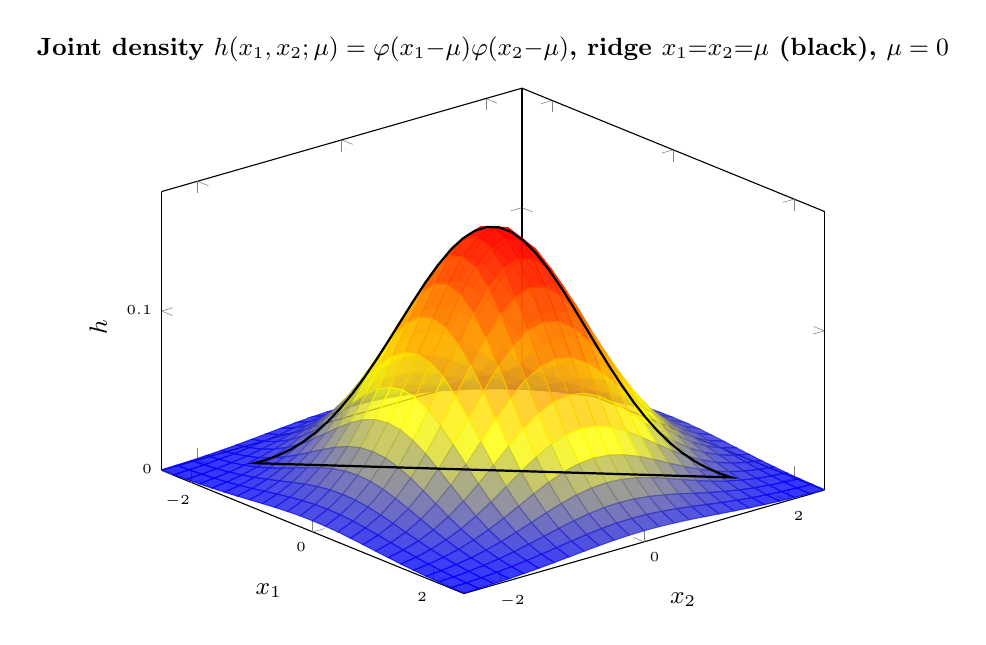
\begin{tikzpicture}
\begin{axis}[
  width=10cm, height=8cm,
  xlabel={$x_1$}, ylabel={$x_2$}, zlabel={$h$},
  title={Joint density $h(x_1,x_2;\mu)=\varphi(x_1{-}\mu)\varphi(x_2{-}\mu)$,\
    ridge $x_1{=}x_2{=}\mu$ (black), $\mu=0$},
  xmin=-2.5, xmax=2.5, ymin=-2.5, ymax=2.5, zmin=0, zmax=0.175,
  domain=-2.5:2.5, y domain=-2.5:2.5, samples=25,
  view={50}{30},
  colormap/hot,
  title style={font=\small\bfseries},
  label style={font=\small},
  tick label style={font=\tiny},
]
\addplot3[surf,opacity=0.80,shader=flat corner]
  {exp(-x^2/2)/sqrt(2*3.14159) * exp(-y^2/2)/sqrt(2*3.14159)};
% diagonal ridge x1=x2=mu (peak)
\addplot3[thick,black,domain=-1.8:1.8,samples=40]
  (x, x, {(exp(-x^2/2)/sqrt(2*3.14159))^2});
\end{axis}
\end{tikzpicture}
\end{center}

\begin{center}
\begin{center}
\includegraphics[width=0.60\textwidth]{fig_so_n2_density.png}
\end{center}

\begin{center}
\includegraphics[width=0.82\textwidth]{fig_so_n2_paraboloid.png}
\end{center}
\end{center}

\paragraph{Step 10.\ Differentiating in $\mu$: the sample mean appears.}
Differentiate the joint log-likelihood:
\[
  s(\mathbf{x}, \mu)
  \;=\; \frac{\partial}{\partial\mu}\,\ell(\mathbf{x}, \mu)
  \;=\; -\tfrac{1}{2}\sum_{i=1}^n \frac{\partial}{\partial\mu}(x_i - \mu)^2
  \;=\; \sum_{i=1}^n (x_i - \mu)
  \;=\; n\bar x - n\mu
  \;=\; n(\bar x - \mu),
\]
where $\bar x = \tfrac{1}{n}\sum_i x_i$ is the sample mean.  Two
observations are worth flagging.

\begin{itemize}
\item \textbf{The pre-score is additive over the sample.}  The
  joint pre-score is the sum of the individual pre-scores
  $s(x_i, \mu) = x_i - \mu$.  This is the operator-algebra of $D$
  applied to the product $h = \prod \varphi(x_i - \mu)$:
  multiplication of densities becomes addition of pre-scores
  (Property~1 of the semi-elasticity section (Part~2)).

\item \textbf{The pre-score factors through $\bar x$.}  The joint
  pre-score $n(\bar x - \mu)$ depends on the data only through
  $\bar x$.  Equivalently, $\ell(\mathbf{x}, \mu)$ can be written
  as $\tilde\ell(\bar x(\mathbf{x}), \mu)$ for some function
  $\tilde\ell : \mathbb{R}^2 \to \mathbb{R}$.  The sample mean is
  a \emph{sufficient statistic} for $\mu$ in this family.  This is
  the entry point to sufficiency theory; we do not pursue it here.
\end{itemize}

\begin{center}
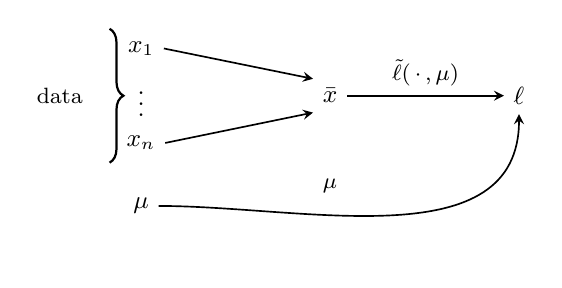
\begin{tikzpicture}[font=\small,
  arr/.style={->,>=stealth,semithick},
  box/.style={draw=none}]
% left column: x1 ... xn
\node[box] (x1) at (0, 1.2)  {$x_1$};
\node[box]       at (0, 0.6)  {$\vdots$};
\node[box] (xn) at (0, 0.0)  {$x_n$};
% xbar node
\node[box] (xb) at (2.4, 0.6) {$\bar x$};
% ell node
\node[box] (el) at (4.8, 0.6) {$\ell$};
% mu node (below left)
\node[box] (mu) at (0, -0.8)  {$\mu$};
% arrows: x1,xn → xbar
\draw[arr] (x1.east) -- (xb.north west);
\draw[arr] (xn.east) -- (xb.south west);
% arrow: xbar → ell
\draw[arr] (xb) -- (el) node[midway,above,font=\footnotesize]
  {$\tilde\ell(\,\cdot\,,\mu)$};
% arrow: mu → ell (long, curved below)
\draw[arr] (mu.east) to[out=0,in=270] (el.south)
  node[pos=0.55,below,font=\footnotesize] {};
\node[font=\footnotesize] at (2.4,-0.55) {$\mu$};
% brace label
\draw[decorate,decoration={brace,amplitude=5pt,mirror},thick]
  (-0.4,-0.25) -- (-0.4,1.45)
  node[midway,left=6pt,font=\footnotesize] {data};
\end{tikzpicture}
\end{center}

\begin{center}
\includegraphics[width=0.65\textwidth]{fig_so_sufficiency.png}
\end{center}

\begin{remark}[The role of $\mu$]
At this stage $\mu$ is a free variable, not the true parameter.
We are differentiating $\ell$ with respect to $\mu$ as a function
of two arguments; the result $s(\mathbf{x}, \mu) = n(\bar x - \mu)$
is the pre-score, a function of both.  When we later substitute a
\emph{specific} value $\mu = \mu_0$ (the true parameter) and treat
$\mathbf{x}$ as random under $\mathcal{N}(\mu_0, 1)$, the same
expression becomes a random variable whose distribution we will
compute.
\end{remark}

\paragraph{Step 11.\ The score identity $\E_\mu[s] = 0$, in three rounds.}
We verify $\E_\mu[s(\mathbf{X}, \mu)] = 0$ directly by integration,
in three rounds of increasing complexity.

\textbf{Round 1: $n=1$, general parametric family.}
Starting from the definition $s = \partial_\theta\!\log f_\theta =
\partial_\theta f_\theta / f_\theta$ and using Path B of the
semi-elasticity operator,
\[
  \E_\theta[s(X,\theta)]
  \;=\; \int_{\mathbb{R}} s(x,\theta)\,f_\theta(x)\,dx
  \;=\; \int \frac{\partial_\theta f_\theta(x)}{f_\theta(x)}\cdot f_\theta(x)\,dx
  \;=\; \int \partial_\theta f_\theta(x)\,dx
  \;=\; 0,
\]
the last equality being Property~3 of
the Density and Likelihood chapter (Part~2).  The denominator $f_\theta$
in the score cancels against the density used to take expectation.
This is the general route; it works for any sufficiently regular
family.

\textbf{Round 2: $n=1$, normal family --- explicit calculation.}
For $\mathcal{N}(\mu, 1)$, work the same identity by direct
substitution.  First a side calculation: the derivative of $\varphi$
in its argument is
\[
  \varphi'(x) \;=\; \frac{1}{\sqrt{2\pi}}\,
  \frac{d}{dx}e^{-x^2/2}
  \;=\; \frac{1}{\sqrt{2\pi}}\,e^{-x^2/2}\cdot(-x)
  \;=\; -x\,\varphi(x).
\]
So $\varphi'$ is the reflected curve $-x\,\varphi(x)$ --- positive
for $x<0$, negative for $x>0$.

\begin{center}
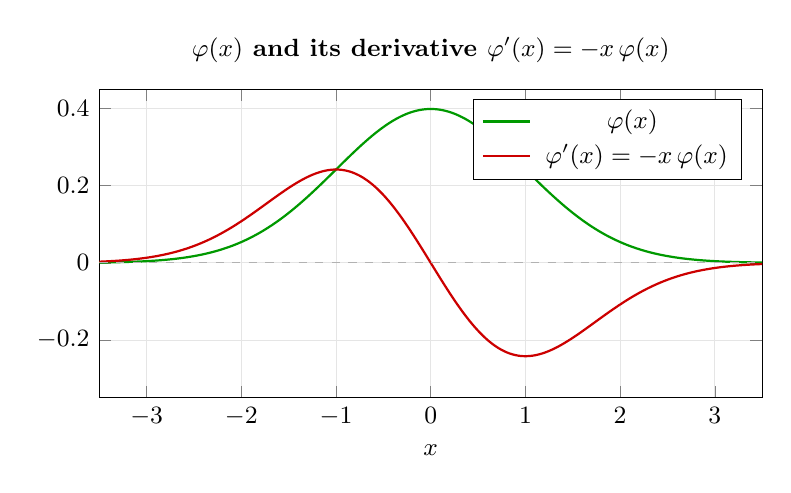
\begin{tikzpicture}
\begin{axis}[
  width=10cm, height=5.5cm,
  xlabel={$x$},
  title={$\varphi(x)$ and its derivative $\varphi'(x)=-x\,\varphi(x)$},
  xmin=-3.5, xmax=3.5, ymin=-0.35, ymax=0.45,
  domain=-3.5:3.5, samples=200,
  grid=both, grid style={line width=0.3pt,draw=gray!20},
  tick label style={font=\small},
  title style={font=\small\bfseries},
  label style={font=\small},
  legend pos=north east, legend style={font=\small},
]
\addplot[thick,green!60!black]{exp(-x^2/2)/sqrt(2*3.14159)};
\addplot[thick,red!80!black]{-x*exp(-x^2/2)/sqrt(2*3.14159)};
\addplot[dashed,gray!60] coordinates {(-3.5,0)(3.5,0)};
\legend{$\varphi(x)$,\ $\varphi'(x)=-x\,\varphi(x)$}
\end{axis}
\end{tikzpicture}
\end{center}

\begin{center}
\includegraphics[width=0.60\textwidth]{fig_so_phi_deriv.png}
\end{center}

Then for $\varphi_\mu(x) =
\varphi(x-\mu)$, the chain rule in $\mu$ gives
\[
  \frac{\partial}{\partial\mu}\,\varphi(x-\mu)
  \;=\; \varphi'(x-\mu)\cdot \frac{\partial}{\partial\mu}(x-\mu)
  \;=\; -(x-\mu)\,\varphi(x-\mu)\cdot(-1)
  \;=\; (x-\mu)\,\varphi(x-\mu).
\]
Taking the expectation,
\[
  \E_\mu[s(X,\mu)]
  \;=\; \int (x-\mu)\,\varphi(x-\mu)\,dx
  \;=\; \int_{-\infty}^{\infty} y\,\varphi(y)\,dy
  \;=\; 0,
\]
by the substitution $y = x-\mu$ and the symmetry of the standard
normal.  The score identity is realised as the first moment of a
standard normal being zero --- a clean concrete answer.

\textbf{Round 3: $n>1$, normal family --- factorisation.}
For the i.i.d.\ sample,
\[
  h(x_1,\ldots,x_n;\mu) \;=\; \prod_{i=1}^n \varphi(x_i - \mu),
\]
and differentiating in $\mu$ gives
\[
  \frac{\partial h}{\partial\mu}
  \;=\; \sum_{i=1}^n (x_i-\mu)\,\varphi(x_i-\mu)\,\prod_{j\neq i}\varphi(x_j-\mu).
\]
(Here we are computing $\partial_\mu h$ to use Path B; equivalently
one can compute $\partial_\mu \ell = n(\bar x - \mu)$ and multiply
back by $h$.)  Taking the expectation under $\mathcal{N}(\mu,1)^n$:
\[
  \E_\mu[s(\mathbf{X},\mu)]
  \;=\; \int \cdots \int
  \sum_{i=1}^n (x_i-\mu)\,\prod_{j=1}^n \varphi(x_j-\mu)\,dx_1\cdots dx_n.
\]
By independence the multidimensional integral factorises into a sum
of products.  For the $i$-th term, the integrals over $x_j$ with
$j\neq i$ each give $1$ (densities integrate to one), and the
integral over $x_i$ is
$\int (x_i-\mu)\,\varphi(x_i-\mu)\,dx_i = 0$ by Round~2.  Every
term in the sum vanishes individually:
\[
  \E_\mu[s] \;=\; \underbrace{0 + 0 + \cdots + 0}_{n \text{ terms}}
  \;=\; 0.
\]

\paragraph{What this verification shows.}
The score identity holds at all three levels --- general parametric,
specific normal $n=1$, specific normal $n>1$ --- by different but
parallel arguments.  The general argument is the denominator
cancellation (Round 1).  The specific normal $n=1$ argument is the
symmetry of the bell (Round 2).  The $n>1$ argument is the
factorisation due to i.i.d.\ structure, reducing to $n$ copies of
Round 2 (Round 3).

\paragraph{What we have now built.}
At the end of the Score and Fisher Information chapter (Part~2), the
$\mathcal{N}(\mu, 1)$ example has been carried through every
construction: density, pre-likelihood, log-likelihood, the random
indexing via $\omega$, the cloud of parabolas in finite samples,
the pre-score factoring through $\bar x$, sufficiency, and the
score identity verified three ways.  The same machinery applied to
test $H_0: \mu = \mu_0$ in three different ways (Wald, LR, score)
in the next chapter, and explains why they asymptotically agree.


%--------------------------------------------------------------------
\subsection{MLE for $\mathcal{N}(\mu,1)$: finding the argmax}
\label{sec:mle_normal}
%--------------------------------------------------------------------

We now apply the machinery of the previous two subsections to find
the MLE explicitly.  The question is: given data, which value of
$\mu$ maximises the likelihood?  We answer it first for $n=1$, where
the geometry is transparent, and then for general $n$, where the
sample mean emerges as a sufficient reduction.

%--------------------------------------------------------------------
\paragraph{Case $n=1$.}
Fix $x = x_1$ and maximise $h(x_1,\mu) = \varphi(x_1 - \mu)$ over
$\mu$.  The bivariate surface $h(x,\mu)$ was drawn in Step~3; the
MLE is the point on that surface directly above the diagonal ridge
$x = \mu$.  Cutting the surface with the vertical plane $x = x_1$
(the \emph{red slice} in the figure below) gives the pre-likelihood
$L_{x_1}(\mu) = \varphi(x_1 - \mu)$ as a function of $\mu$ alone.

\begin{center}
\includegraphics[width=0.82\textwidth]{fig_mle_3d_hand.png}
\end{center}

\noindent The red slice is itself a bell curve in $\mu$, centred at
$\mu = x_1$:

\begin{center}
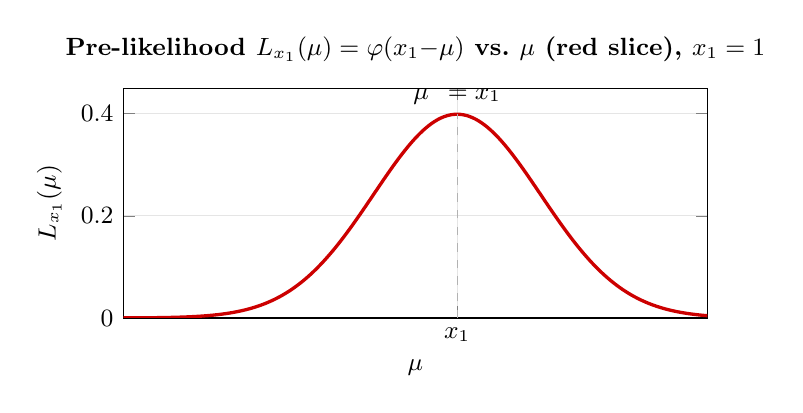
\begin{tikzpicture}
\begin{axis}[
  width=9cm, height=4.5cm,
  xlabel={$\mu$}, ylabel={$L_{x_1}(\mu)$},
  title={Pre-likelihood $L_{x_1}(\mu)=\varphi(x_1{-}\mu)$
    vs.\ $\mu$ (red slice), $x_1=1$},
  xmin=-3, xmax=4, ymin=0, ymax=0.45,
  domain=-3:4, samples=200,
  grid=both, grid style={line width=0.3pt,draw=gray!20},
  tick label style={font=\small},
  title style={font=\small\bfseries,align=center},
  label style={font=\small},
  xtick={1}, xticklabels={$x_1$},
]
\addplot[very thick,red!80!black]{exp(-(x-1)^2/2)/sqrt(2*3.14159)};
\addplot[dashed,gray!60] coordinates {(1,0)(1,0.4)};
\node[font=\small,anchor=south] at (axis cs:1,0.40) {$\mu^*=x_1$};
\end{axis}
\end{tikzpicture}
\end{center}

\noindent Taking the log converts the bell into a downward parabola,
whose vertex is still at $\mu^* = x_1$:
\[
  \ell_{x_1}(\mu) \;=\; \log\varphi(x_1-\mu)
  \;=\; -\tfrac{1}{2}(x_1-\mu)^2 - \tfrac{1}{2}\log(2\pi).
\]

\begin{center}
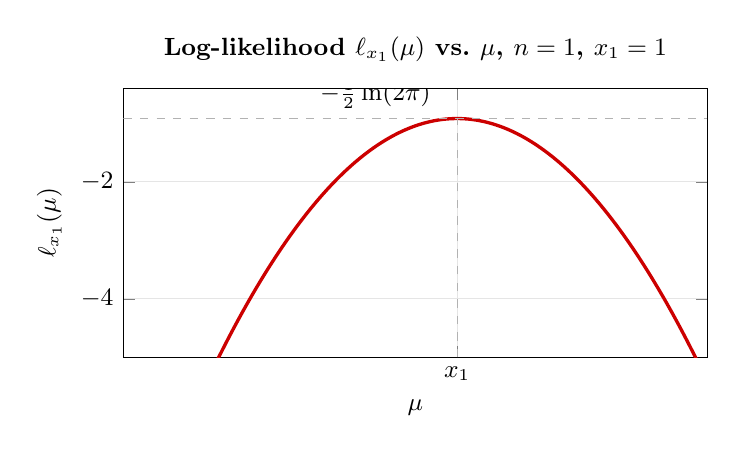
\begin{tikzpicture}
\begin{axis}[
  width=9cm, height=5cm,
  xlabel={$\mu$}, ylabel={$\ell_{x_1}(\mu)$},
  title={Log-likelihood $\ell_{x_1}(\mu)$ vs.\ $\mu$, $n=1$, $x_1=1$},
  xmin=-3, xmax=4, ymin=-5, ymax=-0.4,
  domain=-3:4, samples=200,
  grid=both, grid style={line width=0.3pt,draw=gray!20},
  tick label style={font=\small},
  title style={font=\small\bfseries},
  label style={font=\small},
  xtick={1}, xticklabels={$x_1$},
]
\addplot[very thick,red!80!black]{-(x-1)^2/2 - 0.919};
\addplot[dashed,gray!60] coordinates {(1,-5)(1,-0.919)};
\addplot[dashed,gray!60] coordinates {(-3,-0.919)(4,-0.919)};
\node[font=\small,anchor=south east] at (axis cs:0.8,-0.919)
  {$-\tfrac{1}{2}\ln(2\pi)$};
\node[font=\small,anchor=south] at (axis cs:1,-0.4)
  {$\mu^*=x_1$};
\end{axis}
\end{tikzpicture}
\end{center}

The MLE for $n=1$ is $\hat\mu = x_1$: the single observation is the
maximum-likelihood guess for the location.

%--------------------------------------------------------------------
\paragraph{Case $n=2$: the 3D picture and its limitation.}
For two observations $(x_1,x_2)$ the joint log-likelihood is
\[
  \ell(x_1,x_2;\mu)
  \;=\; -\tfrac{1}{2}(x_1-\mu)^2 - \tfrac{1}{2}(x_2-\mu)^2 - \ln(2\pi),
\]
which was visualised as a downward paraboloid in $(x_1,x_2,\ell)$-space
in Step~9 (the red bowl on page~41).  However, that picture is a
function of all three variables simultaneously: it is \emph{not}
useful for visualising the MLE, which requires holding $(x_1,x_2)$
fixed and varying $\mu$ alone.

%--------------------------------------------------------------------
\paragraph{Case $n\geq 1$: reduction to $Q(\mu)$.}
For a general i.i.d.\ sample $(x_1,\ldots,x_n)$ write out the
exponent:
\[
  Q(x_1,\ldots,x_n;\mu)
  \;:=\; \sum_{i=1}^n(x_i-\mu)^2
  \;=\; \sum x_i^2 + n\mu^2 - 2\mu\sum x_i
  \;=\; n\bigl(\mu^2 - 2\bar x\,\mu + \overline{x^2}\bigr)
  \;=\; \tilde Q(n,\mu,\bar x, \overline{x^2}),
\]
where $\bar x = \frac{1}{n}\sum x_i$ and $\overline{x^2} =
\frac{1}{n}\sum x_i^2$.  The joint density factors as
\[
  h(\mathbf{x};\mu)
  \;=\; C\cdot e^{-\frac{1}{2}Q(\mathbf{x};\mu)},
\]
so $\operatorname{argmax}_\mu h = \operatorname{argmin}_\mu Q$.

\medskip
\noindent\textbf{Key observation.}  Although $Q$ depends on the data
through \emph{both} $\bar x$ and $\overline{x^2}$, the argmin in $\mu$
depends only on $\bar x$.  Concretely, treating $Q/n$ as a function
of $\mu$ alone:
\[
  \frac{Q}{n} \;=\; \mu^2 - 2\bar x\,\mu + \overline{x^2},
  \qquad
  \frac{d}{d\mu}\!\left(\frac{Q}{n}\right) \;=\; 2\mu - 2\bar x \;=\; 0
  \;\;\Longrightarrow\;\; \mu^* \;=\; \bar x.
\]

For fixed $(x_1,x_2)$ the log-likelihood $\ell_{x_1,x_2}(\mu)$ is
therefore a downward parabola in $\mu$ alone, with vertex at $\bar x
= (x_1+x_2)/2$:

\begin{center}
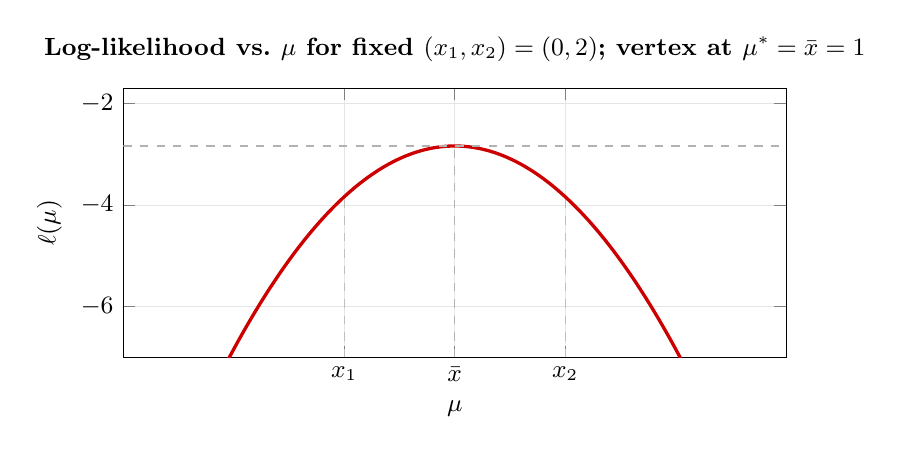
\begin{tikzpicture}
\begin{axis}[
  width=10cm, height=5cm,
  xlabel={$\mu$}, ylabel={$\ell(\mu)$},
  title={Log-likelihood vs.\ $\mu$ for fixed $(x_1,x_2)=(0,2)$;
    vertex at $\mu^*=\bar x=1$},
  xmin=-2, xmax=4, ymin=-7, ymax=-1.7,
  domain=-2:4, samples=200,
  grid=both, grid style={line width=0.3pt,draw=gray!20},
  tick label style={font=\small},
  title style={font=\small\bfseries,align=center},
  label style={font=\small},
  xtick={0,1,2}, xticklabels={$x_1$,$\bar x$,$x_2$},
]
% ell(mu) = -1/2*(0-mu)^2 - 1/2*(2-mu)^2 - ln(2pi)
%         = -1/2*(mu^2 + (mu-2)^2) - 1.838
%         = -(mu^2 - 2mu + 2) - 1.838 (simplify: mu^2-2mu+2 = (mu-1)^2+1)
% = -(mu-1)^2 - 1 - 1.838 = -(mu-1)^2 - 2.838
\addplot[very thick,red!80!black]{-(x-1)^2 - 2.838};
\addplot[dashed,gray!60] coordinates {(1,-7)(1,-2.838)};
\addplot[dashed,gray!60] coordinates {(-2,-2.838)(4,-2.838)};
\addplot[dashed,gray!50] coordinates {(0,-7)(0,-3.838)};
\addplot[dashed,gray!50] coordinates {(2,-7)(2,-3.838)};
\node[font=\small,anchor=south] at (axis cs:1,-1.7) {$\mu^*=\bar x$};
\node[font=\small,anchor=west] at (axis cs:4,-2.838)
  {$-\ln(2\pi)-1$};
\end{axis}
\end{tikzpicture}
\end{center}

\noindent\textbf{Summary.}  The likelihood depends on the data
through both $\bar x$ and $\overline{x^2}$, but its argmax depends
only on $\bar x$, and equals $\bar x$.  This is the sample mean as
MLE.



%====================================================================
\subsection{Fisher information for $\mathcal{N}(\mu,1)$}
%====================================================================

%--------------------------------------------------------------------
\paragraph{Definition.}

The \emph{Fisher information} is the variance of the score:
\[
  \mathcal{I}(\theta)
  \;=\; \mathrm{Var}_\theta\bigl[s(X,\theta)\bigr]
  \;=\; \E_\theta\!\left[\left(\frac{\partial}{\partial\theta}
        \log f(X;\theta)\right)^{\!2}\right]
  \;=\; \int_{\mathbb{R}}
        \!\left(\frac{\partial}{\partial\theta}\log f(x;\theta)\right)^{\!2}
        f(x;\theta)\,dx,
\]
where the last equality holds under absolute continuity (Lebesgue density
exists).  Since $\mathcal{I}(\theta)$ is the expectation of a square, it
is always non-negative.

Structurally, $\mathcal{I}$ is an operator on one-parametric families of
measures: $\{P_\theta\}_{\theta\in\Theta} \mapsto \mathcal{I}(\cdot)$,
where $\mathcal{I}(\cdot)\colon\Theta\to\mathbb{R}$.  The parameter space
$\Theta$ must be a continuum (e.g.\ an interval) because we need to
differentiate in $\theta$.  The first picture shows the case of a finite
parameter set $\Theta=\{\theta_1,\theta_2,\theta_3\}$ as a toy illustration:
a family of measures on the left maps to three scalar values on the right.

\begin{center}
\includegraphics[width=0.80\textwidth]{fi_fig1_operator_discrete.png}
\end{center}

When $\Theta$ is a continuum the family of measures is harder to depict,
but the output function $\mathcal{I}(\cdot)$ is easy --- it is just a
curve over $\theta$:

\begin{center}
\includegraphics[width=0.80\textwidth]{fi_fig2_operator_continuous.png}
\end{center}

%--------------------------------------------------------------------
\paragraph{Two routes to $\mathcal{I}$: generic vs.\ regular.}

In the generic (absolutely continuous) case:
\begin{enumerate}
\item Square the score $s(x,\theta)$.
\item Integrate against the density $f_\theta(x)$.
\end{enumerate}
Under \emph{regularity conditions} (differentiation under the integral
sign is valid) a third equivalent formula holds:
\[
  \mathcal{I}(\theta)
  \;=\; -\E_\theta\!\left[\frac{\partial^2}{\partial\theta^2}
        \ln L_x(\theta)\right]
  \;=\; -\E_\theta\!\left[\frac{\partial}{\partial\theta}s_x(\theta)\right].
\]
This adds a differentiation and a negation step:
\begin{enumerate}
\item Differentiate the score in $\theta$.
\item Integrate against $f_\theta$.
\item Negate.
\end{enumerate}
We work out both for $\mathcal{N}(\mu,1)$.

%--------------------------------------------------------------------
\paragraph{Score for $\mathcal{N}(\mu,1)$.}

For the location family $f_\mu(x) = \varphi(x-\mu)$:
\[
  \ell_x(\mu) \;=\; -\tfrac{1}{2}\ln(2\pi) - \tfrac{1}{2}(x-\mu)^2,
  \qquad
  s_x(\mu) \;=\; \frac{\partial \ell_x}{\partial\mu} \;=\; x-\mu.
\]
The pre-integrand for the generic formula is $(x-\mu)^2$ --- just a
square.  The bivariate surface $s(x,\mu)=x-\mu$ over the $(x,\mu)$-plane:

\begin{center}
\includegraphics[width=0.82\textwidth]{fi_fig3_score_surface_3d.png}
\end{center}

Fix $\mu=\mu_0$.  The green density $\varphi(x-\mu_0)$ is added as a
section:

\begin{center}
\includegraphics[width=0.82\textwidth]{fi_fig4_score_3d_mu0.png}
\end{center}

%--------------------------------------------------------------------
\paragraph{Forming the pre-integral curve.}

The 2D picture at fixed $\mu_0$ shows the squared score $(x-\mu_0)^2$
(green) and the density $\varphi(x-\mu_0)$ (black) side by side:

\begin{center}
\includegraphics[width=0.78\textwidth]{fi_fig5_score_sq_2d.png}
\end{center}

Multiplying them gives the pre-integral curve (red):
$(x-\mu_0)^2\cdot\varphi(x-\mu_0)$:

\begin{center}
\includegraphics[width=0.78\textwidth]{fi_fig6_preintegral_2d.png}
\end{center}

%--------------------------------------------------------------------
\paragraph{Computing $\mathcal{I}_{\mathcal{N}(\mu,1)}(\mu)$.}

Integrating with the substitution $y=x-\mu$:
\[
  \mathcal{I}_{\mathcal{N}(\mu,1)}(\mu)
  \;=\; \int_{-\infty}^{\infty}(x-\mu)^2\,\varphi(x-\mu)\,dx
  \;=\; \int_{-\infty}^{\infty}y^2\,\varphi(y)\,dy
  \;=\; \mathrm{Var}(Z) \;=\; 1, \quad Z\sim\mathcal{N}(0,1).
\]
The result does not depend on $\mu$ --- $\mathcal{I}$ is constant for
this family:

\begin{center}
\includegraphics[width=0.55\textwidth]{fi_fig7_fisher_flat.png}
\end{center}

This constancy is specific to the location-normal family.  In general
$\mathcal{I}(\theta)$ depends on $\theta$.

%--------------------------------------------------------------------
\paragraph{Regular formula: differentiating the score.}

For the regular formula we need $\frac{\partial}{\partial\mu}s(x,\mu)$.
Here $s(x,\mu)=x-\mu$, so:
\[
  \frac{\partial}{\partial\mu}s(x,\mu)
  \;=\; \frac{\partial}{\partial\mu}(x-\mu) \;=\; -1.
\]
Already at this level the derivative does not depend on $x$.
The 2D section at a fixed $\mu$ (the score as a function of $x$):

\begin{center}
\includegraphics[width=0.55\textwidth]{fi_fig8_score_2d_fixed_mu.png}
\end{center}

The bivariate surface $\partial_\mu s(x,\mu)\equiv -1$ is a flat
horizontal plane at height $-1$ over the entire $(x,\mu)$-plane:

\begin{center}
\includegraphics[width=0.82\textwidth]{fi_fig9_dscore_3d.png}
\end{center}

\begin{center}
\includegraphics[width=0.82\textwidth]{fi_fig10_dscore_3d_b.png}
\end{center}

%--------------------------------------------------------------------
\paragraph{Sections of $\partial_\mu s \equiv -1$.}

The flat plane is also shown alone, then its 2D sections:

\begin{center}
\includegraphics[width=0.82\textwidth]{fi_fig11_dscore_plane.png}
\end{center}

Section at fixed $\mu=\mu_1$ (as a function of $x$): a horizontal
line at $-1$:

\begin{center}
\includegraphics[width=0.65\textwidth]{fi_fig12_section_mu.png}
\end{center}

Section at fixed $x=x_1$ (as a function of $\mu$): also a horizontal
line at $-1$:

\begin{center}
\includegraphics[width=0.65\textwidth]{fi_fig13_section_x.png}
\end{center}

%--------------------------------------------------------------------
\paragraph{Forming the product and negating.}

The product $\frac{\partial}{\partial\mu}s(x,\mu)\cdot f_\mu(x)
= (-1)\cdot\varphi(x-\mu) = -\varphi(x-\mu)$
at $\mu=\mu_1$ is the negative density --- an upside-down bell curve:

\begin{center}
\includegraphics[width=0.78\textwidth]{fi_fig14_neg_phi.png}
\end{center}

Negating gives $\varphi(x-\mu)$, which integrates to $1$ by Lebesgue:

\begin{center}
\includegraphics[width=0.78\textwidth]{fi_fig15_phi_pos.png}
\end{center}

\[
  \mathcal{I}(\mu)
  \;=\; -\int_{-\infty}^{\infty}
        \frac{\partial}{\partial\mu}s(x,\mu)\cdot\varphi(x-\mu)\,dx
  \;=\; \int_{-\infty}^{\infty}\varphi(x-\mu)\,dx \;=\; 1.
\]
Both routes confirm $\mathcal{I}_{\mathcal{N}(\mu,1)}\equiv 1$.

%====================================================================

\end{document}
